\documentclass[]{article}
\usepackage{lmodern}
\usepackage{amssymb,amsmath}
\usepackage{ifxetex,ifluatex}
\usepackage{fixltx2e} % provides \textsubscript
\ifnum 0\ifxetex 1\fi\ifluatex 1\fi=0 % if pdftex
  \usepackage[T1]{fontenc}
  \usepackage[utf8]{inputenc}
\else % if luatex or xelatex
  \ifxetex
    \usepackage{mathspec}
  \else
    \usepackage{fontspec}
  \fi
  \defaultfontfeatures{Ligatures=TeX,Scale=MatchLowercase}
\fi
% use upquote if available, for straight quotes in verbatim environments
\IfFileExists{upquote.sty}{\usepackage{upquote}}{}
% use microtype if available
\IfFileExists{microtype.sty}{%
\usepackage{microtype}
\UseMicrotypeSet[protrusion]{basicmath} % disable protrusion for tt fonts
}{}
\usepackage[margin=1.5cm]{geometry}
\usepackage{hyperref}
\hypersetup{unicode=true,
            pdftitle={Atlas-PS 2},
            pdfauthor={David Atlas},
            pdfborder={0 0 0},
            breaklinks=true}
\urlstyle{same}  % don't use monospace font for urls
\usepackage{color}
\usepackage{fancyvrb}
\newcommand{\VerbBar}{|}
\newcommand{\VERB}{\Verb[commandchars=\\\{\}]}
\DefineVerbatimEnvironment{Highlighting}{Verbatim}{commandchars=\\\{\}}
% Add ',fontsize=\small' for more characters per line
\usepackage{framed}
\definecolor{shadecolor}{RGB}{248,248,248}
\newenvironment{Shaded}{\begin{snugshade}}{\end{snugshade}}
\newcommand{\KeywordTok}[1]{\textcolor[rgb]{0.13,0.29,0.53}{\textbf{{#1}}}}
\newcommand{\DataTypeTok}[1]{\textcolor[rgb]{0.13,0.29,0.53}{{#1}}}
\newcommand{\DecValTok}[1]{\textcolor[rgb]{0.00,0.00,0.81}{{#1}}}
\newcommand{\BaseNTok}[1]{\textcolor[rgb]{0.00,0.00,0.81}{{#1}}}
\newcommand{\FloatTok}[1]{\textcolor[rgb]{0.00,0.00,0.81}{{#1}}}
\newcommand{\ConstantTok}[1]{\textcolor[rgb]{0.00,0.00,0.00}{{#1}}}
\newcommand{\CharTok}[1]{\textcolor[rgb]{0.31,0.60,0.02}{{#1}}}
\newcommand{\SpecialCharTok}[1]{\textcolor[rgb]{0.00,0.00,0.00}{{#1}}}
\newcommand{\StringTok}[1]{\textcolor[rgb]{0.31,0.60,0.02}{{#1}}}
\newcommand{\VerbatimStringTok}[1]{\textcolor[rgb]{0.31,0.60,0.02}{{#1}}}
\newcommand{\SpecialStringTok}[1]{\textcolor[rgb]{0.31,0.60,0.02}{{#1}}}
\newcommand{\ImportTok}[1]{{#1}}
\newcommand{\CommentTok}[1]{\textcolor[rgb]{0.56,0.35,0.01}{\textit{{#1}}}}
\newcommand{\DocumentationTok}[1]{\textcolor[rgb]{0.56,0.35,0.01}{\textbf{\textit{{#1}}}}}
\newcommand{\AnnotationTok}[1]{\textcolor[rgb]{0.56,0.35,0.01}{\textbf{\textit{{#1}}}}}
\newcommand{\CommentVarTok}[1]{\textcolor[rgb]{0.56,0.35,0.01}{\textbf{\textit{{#1}}}}}
\newcommand{\OtherTok}[1]{\textcolor[rgb]{0.56,0.35,0.01}{{#1}}}
\newcommand{\FunctionTok}[1]{\textcolor[rgb]{0.00,0.00,0.00}{{#1}}}
\newcommand{\VariableTok}[1]{\textcolor[rgb]{0.00,0.00,0.00}{{#1}}}
\newcommand{\ControlFlowTok}[1]{\textcolor[rgb]{0.13,0.29,0.53}{\textbf{{#1}}}}
\newcommand{\OperatorTok}[1]{\textcolor[rgb]{0.81,0.36,0.00}{\textbf{{#1}}}}
\newcommand{\BuiltInTok}[1]{{#1}}
\newcommand{\ExtensionTok}[1]{{#1}}
\newcommand{\PreprocessorTok}[1]{\textcolor[rgb]{0.56,0.35,0.01}{\textit{{#1}}}}
\newcommand{\AttributeTok}[1]{\textcolor[rgb]{0.77,0.63,0.00}{{#1}}}
\newcommand{\RegionMarkerTok}[1]{{#1}}
\newcommand{\InformationTok}[1]{\textcolor[rgb]{0.56,0.35,0.01}{\textbf{\textit{{#1}}}}}
\newcommand{\WarningTok}[1]{\textcolor[rgb]{0.56,0.35,0.01}{\textbf{\textit{{#1}}}}}
\newcommand{\AlertTok}[1]{\textcolor[rgb]{0.94,0.16,0.16}{{#1}}}
\newcommand{\ErrorTok}[1]{\textcolor[rgb]{0.64,0.00,0.00}{\textbf{{#1}}}}
\newcommand{\NormalTok}[1]{{#1}}
\usepackage{graphicx,grffile}
\makeatletter
\def\maxwidth{\ifdim\Gin@nat@width>\linewidth\linewidth\else\Gin@nat@width\fi}
\def\maxheight{\ifdim\Gin@nat@height>\textheight\textheight\else\Gin@nat@height\fi}
\makeatother
% Scale images if necessary, so that they will not overflow the page
% margins by default, and it is still possible to overwrite the defaults
% using explicit options in \includegraphics[width, height, ...]{}
\setkeys{Gin}{width=\maxwidth,height=\maxheight,keepaspectratio}
\IfFileExists{parskip.sty}{%
\usepackage{parskip}
}{% else
\setlength{\parindent}{0pt}
\setlength{\parskip}{6pt plus 2pt minus 1pt}
}
\setlength{\emergencystretch}{3em}  % prevent overfull lines
\providecommand{\tightlist}{%
  \setlength{\itemsep}{0pt}\setlength{\parskip}{0pt}}
\setcounter{secnumdepth}{0}
% Redefines (sub)paragraphs to behave more like sections
\ifx\paragraph\undefined\else
\let\oldparagraph\paragraph
\renewcommand{\paragraph}[1]{\oldparagraph{#1}\mbox{}}
\fi
\ifx\subparagraph\undefined\else
\let\oldsubparagraph\subparagraph
\renewcommand{\subparagraph}[1]{\oldsubparagraph{#1}\mbox{}}
\fi

%%% Use protect on footnotes to avoid problems with footnotes in titles
\let\rmarkdownfootnote\footnote%
\def\footnote{\protect\rmarkdownfootnote}

%%% Change title format to be more compact
\usepackage{titling}

% Create subtitle command for use in maketitle
\newcommand{\subtitle}[1]{
  \posttitle{
    \begin{center}\large#1\end{center}
    }
}

\setlength{\droptitle}{-2em}
  \title{Atlas-PS 2}
  \pretitle{\vspace{\droptitle}\centering\huge}
  \posttitle{\par}
  \author{David Atlas}
  \preauthor{\centering\large\emph}
  \postauthor{\par}
  \date{}
  \predate{}\postdate{}


\begin{document}
\maketitle

\section{Problem 1}\label{problem-1}

\subsection{a)}\label{a}

Let \(X = (28, 33, 22, 35)\) be our set of i.i.d data points. The
function \(s_p(\theta)=\sqrt{\Sigma_{x \in X}(\theta - x)^2}\), or the
sum of squared residuals.

\subsection{b)}\label{b}

\(s_p(\theta)\) is plotted below, with the R code used to generate the
plot.

\begin{Shaded}
\begin{Highlighting}[]
\KeywordTok{library}\NormalTok{(latex2exp)}
\NormalTok{x <-}\StringTok{ }\KeywordTok{c}\NormalTok{(}\DecValTok{28}\NormalTok{, }\DecValTok{33}\NormalTok{, }\DecValTok{22}\NormalTok{, }\DecValTok{35}\NormalTok{)}
\NormalTok{s_p <-}\StringTok{ }\NormalTok{function(theta, x)\{}
  \CommentTok{# We implement our function to minimize}
  \KeywordTok{return}\NormalTok{(}\KeywordTok{sqrt}\NormalTok{(}\KeywordTok{sum}\NormalTok{((theta -}\StringTok{ }\NormalTok{x) ^}\StringTok{ }\DecValTok{2}\NormalTok{)))}
\NormalTok{\}}

\CommentTok{# We set up our domain for theta}
\NormalTok{theta_space <-}\StringTok{ }\KeywordTok{seq}\NormalTok{(}\DecValTok{20}\NormalTok{, }\DecValTok{35}\NormalTok{, .}\DecValTok{25}\NormalTok{)}
\CommentTok{# We calculate the function value over the space}
\NormalTok{s_p_theta_space <-}\StringTok{ }\KeywordTok{sapply}\NormalTok{(theta_space, function(theta)\{}\KeywordTok{s_p}\NormalTok{(theta, x)\})}

\CommentTok{# We plot the function over the space}
\KeywordTok{plot}\NormalTok{(theta_space, s_p_theta_space, }\StringTok{'l'}\NormalTok{, }
  \DataTypeTok{main=}\KeywordTok{TeX}\NormalTok{(}\StringTok{'Plot of $s_p(}\CharTok{\textbackslash{}\textbackslash{}}\StringTok{Theta)$'}\NormalTok{), }
  \DataTypeTok{xlab=}\KeywordTok{TeX}\NormalTok{(}\StringTok{'$}\CharTok{\textbackslash{}\textbackslash{}}\StringTok{theta$'}\NormalTok{), }\DataTypeTok{ylab=}\KeywordTok{TeX}\NormalTok{(}\StringTok{'$s_p(}\CharTok{\textbackslash{}\textbackslash{}}\StringTok{theta)$'}\NormalTok{))}
\end{Highlighting}
\end{Shaded}

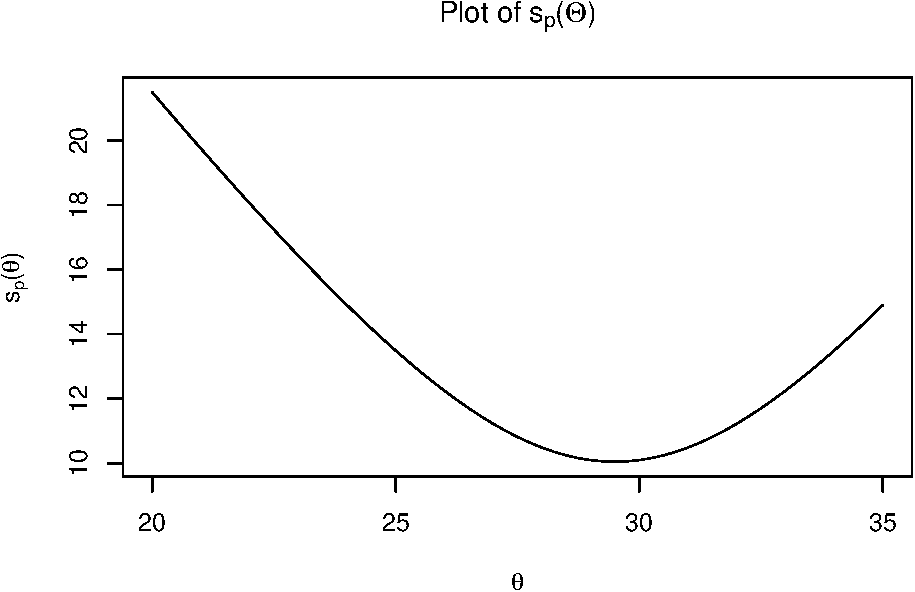
\includegraphics{Atlas-PS_2_files/figure-latex/unnamed-chunk-1-1.pdf}

\subsection{c)}\label{c}

To use the bisection method, we must first compute
\(s_p\prime(\theta)\).

\begin{align*}
  s_p\prime (\theta) &= \frac{1}{2} (\Sigma_{x \in X} (\theta - x)^{2})^{-\frac{1}{2}} \times 2 \Sigma_{x\in X}(\theta-x) \\
  &= (\Sigma_{x \in X} (\theta - x)^{2})^{-\frac{1}{2}} \Sigma_{x\in X}(\theta - x).
\end{align*}

Next, we implement the bisection method, as well as \(s_p(\theta)\) and
\(s_p \prime (\theta)\). We plot the \(s_p(\theta)\) with the Minimum
Residual Estimator as a vertical line. The solution to the optimization
problem is \(\hat{\theta}=29.50\).

\begin{Shaded}
\begin{Highlighting}[]
\NormalTok{x <-}\StringTok{ }\KeywordTok{c}\NormalTok{(}\DecValTok{28}\NormalTok{, }\DecValTok{33}\NormalTok{, }\DecValTok{22}\NormalTok{, }\DecValTok{35}\NormalTok{)}

\NormalTok{s_p <-}\StringTok{ }\NormalTok{function(theta, x)\{}
  \CommentTok{# We implement our function to minimize}
  \KeywordTok{return}\NormalTok{(}\KeywordTok{sqrt}\NormalTok{(}\KeywordTok{sum}\NormalTok{((theta -}\StringTok{ }\NormalTok{x) ^}\StringTok{ }\DecValTok{2}\NormalTok{)))}
\NormalTok{\}}

\NormalTok{s_p_prime <-}\StringTok{ }\NormalTok{function(theta, x)\{}
  \CommentTok{# This is the first derivative of the function}
  \KeywordTok{return}\NormalTok{(((}\KeywordTok{sum}\NormalTok{(theta -}\StringTok{ }\NormalTok{x) ^}\StringTok{ }\DecValTok{2}\NormalTok{) ^}\StringTok{ }\NormalTok{-.}\DecValTok{5}\NormalTok{) *}\StringTok{ }\KeywordTok{sum}\NormalTok{(theta -}\StringTok{ }\NormalTok{x))}
\NormalTok{\}}

\NormalTok{bisection <-}\StringTok{ }\NormalTok{function(a, b, f_prime, }\DataTypeTok{tol=}\NormalTok{.}\DecValTok{0001}\NormalTok{, }\DataTypeTok{n=}\DecValTok{0}\NormalTok{)\{}
  \NormalTok{x_t <-}\StringTok{ }\NormalTok{.}\DecValTok{5} \NormalTok{*}\StringTok{ }\NormalTok{(a +}\StringTok{ }\NormalTok{b)}
  \CommentTok{# Use conditioning to get the next interval}
  \NormalTok{if(}\KeywordTok{f_prime}\NormalTok{(a, x) *}\StringTok{ }\KeywordTok{f_prime}\NormalTok{(x_t, x) <=}\StringTok{ }\DecValTok{0}\NormalTok{)\{}
    \NormalTok{new_interval <-}\StringTok{ }\KeywordTok{c}\NormalTok{(a, x_t)}
  \NormalTok{\}else\{}
    \NormalTok{new_interval <-}\StringTok{ }\KeywordTok{c}\NormalTok{(x_t, b)}
  \NormalTok{\}}
  
  \CommentTok{# if interval is less than the tolerance, stop the recursion.}
  \NormalTok{if ((b -}\StringTok{ }\NormalTok{a) <}\StringTok{ }\NormalTok{tol)\{}
    \KeywordTok{print}\NormalTok{(}\KeywordTok{paste0}\NormalTok{(}\StringTok{"The solution is "}\NormalTok{, }\KeywordTok{round}\NormalTok{(x_t, }\DecValTok{3}\NormalTok{) , }\StringTok{" and it was found in "}\NormalTok{, n, }\StringTok{" iterations."}\NormalTok{))}
    \KeywordTok{return}\NormalTok{(x_t)}
  \NormalTok{\}else\{}
    \CommentTok{# If not, call again on the new interval}
    \KeywordTok{return}\NormalTok{(}\KeywordTok{bisection}\NormalTok{(new_interval[}\DecValTok{1}\NormalTok{], new_interval[}\DecValTok{2}\NormalTok{], f_prime, }\DataTypeTok{n=}\NormalTok{n +}\StringTok{ }\DecValTok{1}\NormalTok{))  }
  \NormalTok{\}}
\NormalTok{\}}

\KeywordTok{plot}\NormalTok{(theta_space, s_p_theta_space, }\StringTok{'l'}\NormalTok{, }
  \DataTypeTok{main=}\KeywordTok{TeX}\NormalTok{(}\StringTok{'Plot of $s_p(}\CharTok{\textbackslash{}\textbackslash{}}\StringTok{Theta)$'}\NormalTok{), }
  \DataTypeTok{xlab=}\KeywordTok{TeX}\NormalTok{(}\StringTok{'$}\CharTok{\textbackslash{}\textbackslash{}}\StringTok{theta$'}\NormalTok{), }\DataTypeTok{ylab=}\KeywordTok{TeX}\NormalTok{(}\StringTok{'$s_p(}\CharTok{\textbackslash{}\textbackslash{}}\StringTok{theta)$'}\NormalTok{))}
\KeywordTok{abline}\NormalTok{(}\DataTypeTok{v=}\KeywordTok{bisection}\NormalTok{(}\DecValTok{20}\NormalTok{, }\DecValTok{35}\NormalTok{, s_p_prime, }\DataTypeTok{tol=}\NormalTok{.}\DecValTok{000001}\NormalTok{))}
\end{Highlighting}
\end{Shaded}

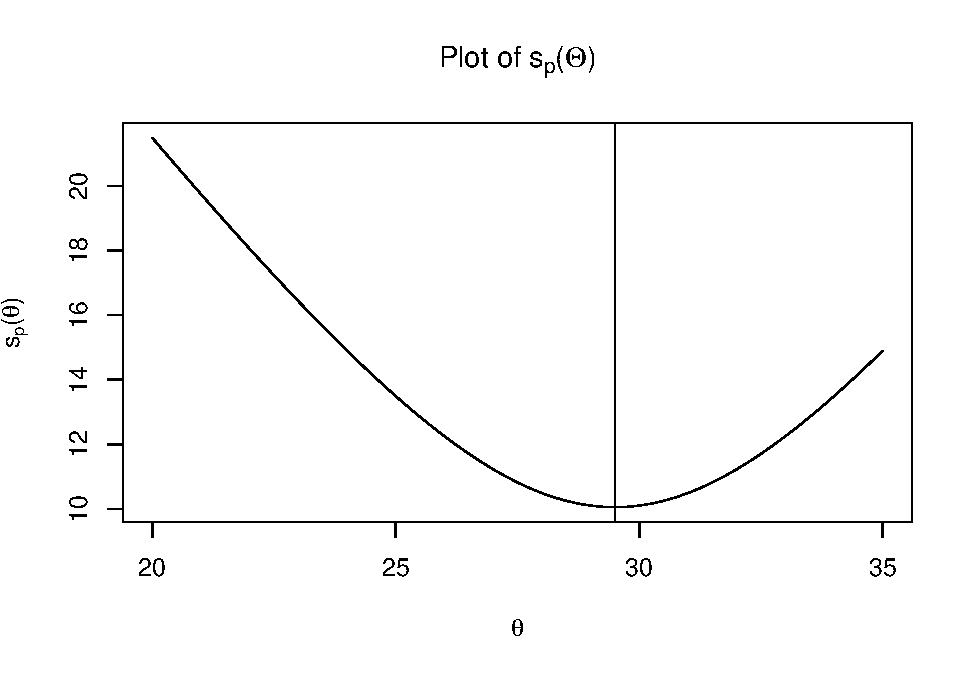
\includegraphics{Atlas-PS_2_files/figure-latex/unnamed-chunk-2-1.pdf}

\begin{verbatim}
## [1] "The solution is 29.5 and it was found in 18 iterations."
\end{verbatim}

\subsection{d)}\label{d}

We already calculated
\(s_p^\prime (\theta) = (\Sigma_{x \in X} (\theta - x)^{2})^{-\frac{1}{2}}\Sigma_{x\in X}(\theta - x)\).
We find

\begin{align*}
s_p^{\prime \prime} (\theta) &= -\frac{1}{2} (\Sigma_{x \in X} (\theta - x)^2)^{-\frac{3}{2}}
\Sigma_{x \in X}(\theta - x) +  (\Sigma_{x \in X} (\theta - x)^2)^{-\frac{1}{2}}.
\end{align*}

We can then find
\(h(\theta) = \frac{s_p^{\prime}(\theta)}{s_p^{\prime \prime}(\theta)}\).

\begin{align*}
  -\frac{s_p^{\prime}(\theta)}{s_p^{\prime \prime}(\theta)} &=
    -\frac{(\Sigma_{x \in X} (\theta - x)^{2})^{-\frac{1}{2}}\Sigma_{x\in X}(\theta - x)}
      {-\frac{1}{2} (\Sigma_{x \in X} (\theta - x)^2)^{-\frac{3}{2}}
      \Sigma_{x \in X}(\theta - x) +  (\Sigma_{x \in X} (\theta - x)^2)^{-\frac{1}{2}}} \\
      &= 2 \frac{\Sigma_{x \in X}(\theta - x)}{\Sigma_{x \in X}(\theta - x)^2 + 2}
\end{align*}

\section{Problem 2}\label{problem-2}

We maximize the function
\(f(x) = -\frac{x^4}{4} + \frac{x^2}{2} - x + 2\) using Newton's Method
and starting points \(x_0=-1\) and \(x_0=2\). We also print out the
number of iterations needed to converge within 2 decimal places. We
define the first 2 derivatives of the function below:

\begin{align}
f(x) &= -\frac{x^4}{4} + \frac{x^2}{2} - x + 2 \\ 
f^{\prime}(x) &= -x^3+ x - 1 \\ 
f^{\prime \prime}(x) &= -3x^2 + 1
\end{align}

We implement Newton's Method:

\begin{Shaded}
\begin{Highlighting}[]
\NormalTok{newtons <-}\StringTok{ }\NormalTok{function(xt, fprime, f2prime, }\DataTypeTok{n=}\DecValTok{1}\NormalTok{, }\DataTypeTok{tol=}\FloatTok{0.01}\NormalTok{)\{}
  \CommentTok{# Define the updating equation}
  \NormalTok{xt_update <-}\StringTok{ }\NormalTok{xt -}\StringTok{ }\NormalTok{(}\KeywordTok{fprime}\NormalTok{(xt) /}\StringTok{ }\KeywordTok{f2prime}\NormalTok{(xt))}
  
  \CommentTok{# If the adjustment value is less than the tolerance, end the iterations}
  \NormalTok{if(}\KeywordTok{abs}\NormalTok{(xt_update -}\StringTok{ }\NormalTok{xt) <}\StringTok{ }\NormalTok{tol)\{}
    \KeywordTok{print}\NormalTok{(}\KeywordTok{paste0}\NormalTok{(}\StringTok{"The solution is "}\NormalTok{, }\KeywordTok{round}\NormalTok{(xt_update, }\DecValTok{3}\NormalTok{) , }\StringTok{" and it was found in "}\NormalTok{, n, }\StringTok{" iterations."}\NormalTok{))}
    \KeywordTok{return}\NormalTok{(xt_update)}
  \NormalTok{\}else\{}
    \CommentTok{# If not, call the recursive formula again}
    \KeywordTok{return}\NormalTok{(}\KeywordTok{newtons}\NormalTok{(xt_update, fprime, f2prime, }\DataTypeTok{n=}\NormalTok{n}\DecValTok{+1}\NormalTok{, }\DataTypeTok{tol=}\NormalTok{tol))}
  \NormalTok{\}}
\NormalTok{\}}

\NormalTok{fprime <-}\StringTok{ }\NormalTok{function(x)\{}
  \KeywordTok{return}\NormalTok{(-x^}\DecValTok{3} \NormalTok{+}\StringTok{ }\NormalTok{x -}\DecValTok{1}\NormalTok{)}
\NormalTok{\}}

\NormalTok{f2prime <-}\StringTok{ }\NormalTok{function(x)\{}
  \KeywordTok{return}\NormalTok{(-}\DecValTok{3} \NormalTok{*}\StringTok{ }\NormalTok{x ^}\StringTok{ }\DecValTok{2} \NormalTok{+}\StringTok{ }\DecValTok{1}\NormalTok{)}
\NormalTok{\}}
\end{Highlighting}
\end{Shaded}

\subsection{a)}\label{a-1}

We solve the optimization using \(x_0=-1\).

\begin{Shaded}
\begin{Highlighting}[]
\NormalTok{x0 <-}\StringTok{ }\NormalTok{-}\DecValTok{1}
\NormalTok{solution <-}\StringTok{ }\KeywordTok{newtons}\NormalTok{(x0, fprime, f2prime)}
\end{Highlighting}
\end{Shaded}

\begin{verbatim}
## [1] "The solution is -1.325 and it was found in 4 iterations."
\end{verbatim}

The solution is -1.325, and it took 4 iterations to find it.

\subsection{b)}\label{b-1}

We solve the optimization using \(x_0=2\).

\begin{Shaded}
\begin{Highlighting}[]
\NormalTok{x0 <-}\StringTok{ }\DecValTok{2}
\NormalTok{solution <-}\StringTok{ }\KeywordTok{newtons}\NormalTok{(x0, fprime, f2prime)}
\end{Highlighting}
\end{Shaded}

\begin{verbatim}
## [1] "The solution is -1.325 and it was found in 64 iterations."
\end{verbatim}

The solution is -1.325, and it took 64 iterations to find it.

\section{Problem 3}\label{problem-3}

We solve exercise 2.1 from the textbook:

The following data are an i.i.d. sample from a Cauchy(\(\theta\), 1)
distribution: 1.77, -.23, 2.76, 3.80, 3.47, 56.75, -1.34, 4.24, -2.44,
3.29, 3.71, -2.40, 4.53, -.07, -1.05, -13.87, -2.53, -1.75, .27, 43.21.

\subsection{a)}\label{a-2}

Graph the log likelihood function. Find the MLE for \(\theta\) using the
Newton-Raphson method. Try the following starting point: -11, -1, 0,
1.5, 4, 4.7, 7, 8, 38. Discuss your results. Is the mean of the data a
good starting point?

The likelihood function of a Cauchy(\(\theta\), 1) distribution: \[
L(\theta) = \prod_{x \in X} \frac{1}
{\pi(1 + (x - \theta) ^ 2)}.
\] Therefore, the log-likelihood is

\begin{align*}
l(\theta) &= \Sigma_{x \in X}\ln\left(\frac{1}{\pi (1 + (x - \theta)^2)}\right) \\&= \Sigma_{x \in X} -\ln(\pi(1  + (x - \theta)^2)) \\
&= - n \ln(\pi) - \Sigma_{x \in X} \ln(1 + (x - \theta) ^ 2),
\end{align*}

where \(n\) is the number of observations in \(X\).

We plot the function below.

\begin{Shaded}
\begin{Highlighting}[]
\NormalTok{X <-}\StringTok{ }\KeywordTok{c}\NormalTok{(}\FloatTok{1.77}\NormalTok{, -.}\DecValTok{23}\NormalTok{, }\FloatTok{2.76}\NormalTok{, }\FloatTok{3.80}\NormalTok{, }\FloatTok{3.47}\NormalTok{, }\FloatTok{56.75}\NormalTok{, -}\FloatTok{1.34}\NormalTok{, }\FloatTok{4.24}\NormalTok{, }
\NormalTok{-}\FloatTok{2.44}\NormalTok{, }\FloatTok{3.29}\NormalTok{, }\FloatTok{3.71}\NormalTok{, -}\FloatTok{2.40}\NormalTok{, }\FloatTok{4.53}\NormalTok{, -.}\DecValTok{07}\NormalTok{, -}\FloatTok{1.05}\NormalTok{, -}\FloatTok{13.87}\NormalTok{, }
\NormalTok{-}\FloatTok{2.53}\NormalTok{, -}\FloatTok{1.75}\NormalTok{, .}\DecValTok{27}\NormalTok{, }\FloatTok{43.21}\NormalTok{)}

\NormalTok{log_likelihood <-}\StringTok{ }\NormalTok{function(theta, x)\{}
  \KeywordTok{return} \NormalTok{(}\KeywordTok{sum}\NormalTok{(}\KeywordTok{dcauchy}\NormalTok{(x, }\DataTypeTok{location=}\NormalTok{theta, }\DataTypeTok{scale=}\DecValTok{1}\NormalTok{, }\DataTypeTok{log=}\OtherTok{TRUE}\NormalTok{)))}
\NormalTok{\}}

\NormalTok{theta_space <-}\StringTok{ }\KeywordTok{seq}\NormalTok{(-}\DecValTok{50}\NormalTok{, }\DecValTok{100}\NormalTok{, .}\DecValTok{5}\NormalTok{)}
\NormalTok{theta_f <-}\StringTok{ }\KeywordTok{sapply}\NormalTok{(theta_space, function(theta)\{}\KeywordTok{log_likelihood}\NormalTok{(theta, X)\})}
\KeywordTok{plot}\NormalTok{(theta_space, theta_f, }\StringTok{'l'}\NormalTok{, }
    \DataTypeTok{main=}\KeywordTok{TeX}\NormalTok{(}\StringTok{'Log-likelihood of Cauchy($}\CharTok{\textbackslash{}\textbackslash{}}\StringTok{theta$, 1)'} \NormalTok{), }
    \DataTypeTok{xlab=}\KeywordTok{TeX}\NormalTok{(}\StringTok{'$}\CharTok{\textbackslash{}\textbackslash{}}\StringTok{theta$'}\NormalTok{), }\DataTypeTok{ylab=}\StringTok{'Log-likelihood'}\NormalTok{)}
\end{Highlighting}
\end{Shaded}

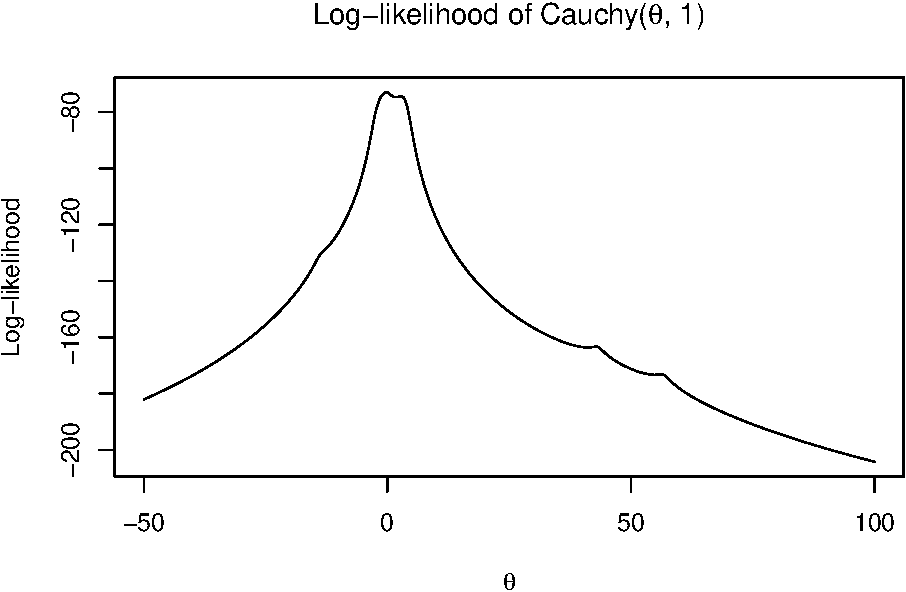
\includegraphics{Atlas-PS_2_files/figure-latex/unnamed-chunk-6-1.pdf} We
note that the log-likelihood values can be negative, as they are not
likelihoods, but rather the natural logarithms of those likelihoods.

Next, we find the MLE for \(\theta\) using Newton's Method for the set
of starting values given above. We calculate the first two derivatives
of the log-likelihood function.

\begin{align*}
l^{\prime} &= - \Sigma_{x \in X} 2 \frac{x - \theta}{1 + (x - \theta) ^2} \\
l^{\prime \prime} &= 
  - \Sigma_{x \in X} 2(1 + (x - \theta)^2)^{-1} + 
    -4 (x - \theta)(1 + (x - \theta)^2)^{-2}(x - \theta) \\
    &= - \Sigma_{x \in X} \frac{2}{1 + (x - \theta)^2} - 
    \frac{4(x - \theta)^2}{(1 + (x - \theta)^2)^2}
\end{align*}

\begin{Shaded}
\begin{Highlighting}[]
\NormalTok{newtons <-}\StringTok{ }\NormalTok{function(xt, fprime, f2prime, }\DataTypeTok{tol=}\FloatTok{0.01}\NormalTok{)\{}
  \CommentTok{# Define the updating equation}
  \NormalTok{n <-}\StringTok{ }\DecValTok{0}
  \NormalTok{xt_update <-}\StringTok{ }\NormalTok{xt +}\StringTok{ }\DecValTok{100}  
  \NormalTok{while(}\KeywordTok{abs}\NormalTok{(}\KeywordTok{fprime}\NormalTok{(xt)) >}\StringTok{ }\NormalTok{tol)\{}
    \NormalTok{xt <-}\StringTok{ }\KeywordTok{ifelse}\NormalTok{(n ==}\StringTok{ }\DecValTok{0}\NormalTok{, xt, xt_update)}
    
    \NormalTok{xt_update <-}\StringTok{ }\NormalTok{xt -}\StringTok{ }\NormalTok{(}\KeywordTok{fprime}\NormalTok{(xt) /}\StringTok{ }\KeywordTok{f2prime}\NormalTok{(xt))}
    \NormalTok{n <-}\StringTok{ }\NormalTok{n +}\StringTok{ }\DecValTok{1}
  \NormalTok{\}}
  \CommentTok{# If the adjustment value is less than the tolerance, end the iterations}
  \KeywordTok{print}\NormalTok{(}\KeywordTok{paste0}\NormalTok{(}\StringTok{"The solution is "}\NormalTok{, }\KeywordTok{round}\NormalTok{(xt_update, }\DecValTok{3}\NormalTok{) , }\StringTok{" and it was found in "}\NormalTok{, n, }\StringTok{" iterations."}\NormalTok{))}
  \KeywordTok{return}\NormalTok{(xt_update)}
\NormalTok{\}}

\NormalTok{fprime <-}\StringTok{ }\NormalTok{function(theta)\{}
  \KeywordTok{return}\NormalTok{(}\DecValTok{2} \NormalTok{*}\StringTok{ }\KeywordTok{sum}\NormalTok{((x-theta) /}\StringTok{ }\NormalTok{(}\DecValTok{1}\NormalTok{+}\StringTok{ }\NormalTok{(x -}\StringTok{ }\NormalTok{theta) ^}\StringTok{ }\DecValTok{2}\NormalTok{)))}
\NormalTok{\}}

\NormalTok{f2prime <-}\StringTok{ }\NormalTok{function(theta)\{}
  
  \NormalTok{secondderivll <-}\StringTok{  }\DecValTok{2} \NormalTok{*}\StringTok{ }\KeywordTok{sum} \NormalTok{(((x -}\StringTok{ }\NormalTok{theta) ^}\StringTok{ }\DecValTok{2} \NormalTok{-}\StringTok{ }\DecValTok{1}\NormalTok{) /}\StringTok{ }\NormalTok{(}\DecValTok{1} \NormalTok{+}\StringTok{ }\NormalTok{(x -}\StringTok{ }\NormalTok{theta) ^}\StringTok{ }\DecValTok{2} \NormalTok{) ^}\StringTok{ }\DecValTok{2}\NormalTok{)}
  \KeywordTok{return}\NormalTok{(secondderivll)  }
  \NormalTok{first_term <-}\StringTok{ }\NormalTok{(}\DecValTok{4} \NormalTok{*}\StringTok{ }\NormalTok{(x -}\StringTok{ }\NormalTok{theta) ^}\StringTok{ }\DecValTok{2}\NormalTok{) /}\StringTok{ }\NormalTok{(}\DecValTok{1} \NormalTok{+}\StringTok{ }\NormalTok{(x -}\StringTok{ }\NormalTok{theta) ^}\StringTok{ }\DecValTok{2}\NormalTok{) ^}\StringTok{ }\DecValTok{2}
  \NormalTok{second_term <-}\StringTok{ }\DecValTok{2} \NormalTok{/}\StringTok{ }\NormalTok{(}\DecValTok{1} \NormalTok{+}\StringTok{ }\NormalTok{(x -}\StringTok{ }\NormalTok{theta) ^}\StringTok{ }\DecValTok{2}\NormalTok{)}
  \KeywordTok{return}\NormalTok{(}\KeywordTok{sum}\NormalTok{(first_term -}\StringTok{ }\NormalTok{second_term))}
\NormalTok{\}}


\NormalTok{starting_points <-}\StringTok{ }\KeywordTok{c}\NormalTok{(-}\DecValTok{11}\NormalTok{, -}\DecValTok{1}\NormalTok{, }\DecValTok{0}\NormalTok{, }\FloatTok{1.5}\NormalTok{, }\DecValTok{4}\NormalTok{, }\FloatTok{4.7}\NormalTok{, }\DecValTok{7}\NormalTok{, }\DecValTok{8}\NormalTok{, }\DecValTok{38}\NormalTok{)}

\NormalTok{solutions <-}\StringTok{ }\KeywordTok{sapply}\NormalTok{(starting_points, function(x0)\{}
  \KeywordTok{print}\NormalTok{(}\KeywordTok{paste0}\NormalTok{(}\StringTok{"Starting Point: "}\NormalTok{, x0))}
  \KeywordTok{newtons}\NormalTok{(x0, }\DataTypeTok{fprime=}\NormalTok{fprime, }\DataTypeTok{f2prime=}\NormalTok{f2prime, }\DataTypeTok{tol=}\NormalTok{.}\DecValTok{01}\NormalTok{)}
\NormalTok{\})}
\end{Highlighting}
\end{Shaded}

\begin{verbatim}
## [1] "Starting Point: -11"
## [1] "The solution is -2507.56 and it was found in 6 iterations."
## [1] "Starting Point: -1"
## [1] "The solution is -1847.745 and it was found in 6 iterations."
## [1] "Starting Point: 0"
## [1] "The solution is -1780.952 and it was found in 6 iterations."
## [1] "Starting Point: 1.5"
## [1] "The solution is -1680.352 and it was found in 6 iterations."
## [1] "Starting Point: 4"
## [1] "The solution is -3052.167 and it was found in 7 iterations."
## [1] "Starting Point: 4.7"
## [1] "The solution is -2956.802 and it was found in 7 iterations."
## [1] "Starting Point: 7"
## [1] "The solution is -2640.641 and it was found in 7 iterations."
## [1] "Starting Point: 8"
## [1] "The solution is -2501.557 and it was found in 7 iterations."
## [1] "Starting Point: 38"
## [1] "The solution is 2999.013 and it was found in 9 iterations."
\end{verbatim}

\begin{Shaded}
\begin{Highlighting}[]
\KeywordTok{plot}\NormalTok{(theta_space, theta_f, }\StringTok{'l'}\NormalTok{, }
    \DataTypeTok{main=}\KeywordTok{TeX}\NormalTok{(}\StringTok{'Log-likelihood of Cauchy($}\CharTok{\textbackslash{}\textbackslash{}}\StringTok{theta$, 1)'} \NormalTok{), }
    \DataTypeTok{xlab=}\KeywordTok{TeX}\NormalTok{(}\StringTok{'$}\CharTok{\textbackslash{}\textbackslash{}}\StringTok{theta$'}\NormalTok{), }\DataTypeTok{ylab=}\StringTok{'Log-likelihood'}\NormalTok{)}

\KeywordTok{abline}\NormalTok{(}\DataTypeTok{v=}\NormalTok{solutions)}
\end{Highlighting}
\end{Shaded}

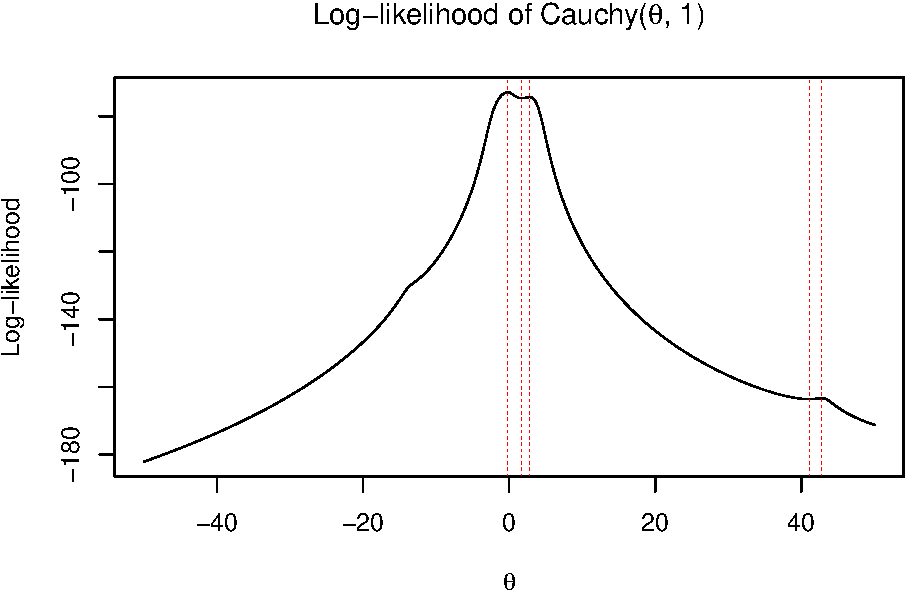
\includegraphics{Atlas-PS_2_files/figure-latex/unnamed-chunk-7-1.pdf}

\subsection{a)}\label{a-3}


\end{document}
